\documentclass[a4paper,12pt]{article}
\usepackage{color}
\usepackage{graphicx, gensymb}
\usepackage{amsfonts, cancel, amssymb}
\usepackage{amsmath, amsthm, array, esvect, esint}
\usepackage{typearea, tikz, pgffor}
\usetikzlibrary{calc, quotes}
\usepackage[a4paper,left=2cm,right=2cm,top=2cm,bottom=3cm,bindingoffset=5mm]{geometry}
\newcommand\numberthis{\addtocounter{equation}{1}\tag{\theequation}}
\newcommand{\bra}{}
\newcommand{\kom}{}
\newcommand{\brak}{}
\newcommand{\braket}{}
\newcommand{\intx}{}
\newcommand{\intr}{}
\newcommand{\kla}{}
\newcommand{\klam}{}
\newcommand{\klammer}{}
\newcommand{\oper}{}
\newcommand{\tecxt}{}
\newcommand{\Bra}{}
\newcommand{\Ket}{}

\begin{document}

\title{02 Strukturanalyse}
\author{Joachim Schwardt}
\date{\today}
\maketitle

\section{Zweidimensionales hexagonales Gitter}
In kartesischen Koordinaten lauten die in (\ref{figure:Hexagonales Gitter mit Gittervektoren}) eingezeichneten Vektoren $\vec{a}_1=(1,0)^\top$ und $\vec{a}_2=(-\frac{1}{2},\frac{\sqrt{3}}{2})^\top$. Sei $A:=(\vec{a}_1\vec{a}_2)=(a_{ij})_{ij}$ die Matrix der Gittervektoren. Dann erhält man die reziproken Gittervektoren aus $b_{ij}=\frac{2\pi}{\det A}\epsilon_{ki}a_{kj}$. In Matrizen ausgedrückt entspricht das
\begin{align*}
B&=\frac{2\pi}{\det A}\begin{pmatrix}
0&-1\\1&0
\end{pmatrix}A=2\pi\begin{pmatrix}
0&-1\\\frac{2}{\sqrt{3}}&-\frac{1}{\sqrt{3}}
\end{pmatrix}
\end{align*}
Die reziproken Vektoren sind mit $\vec{b}_{1,2}$ gekennzeichnet und um einen Faktor 5 verkleinert.
\begin{figure}[h!]
\centering
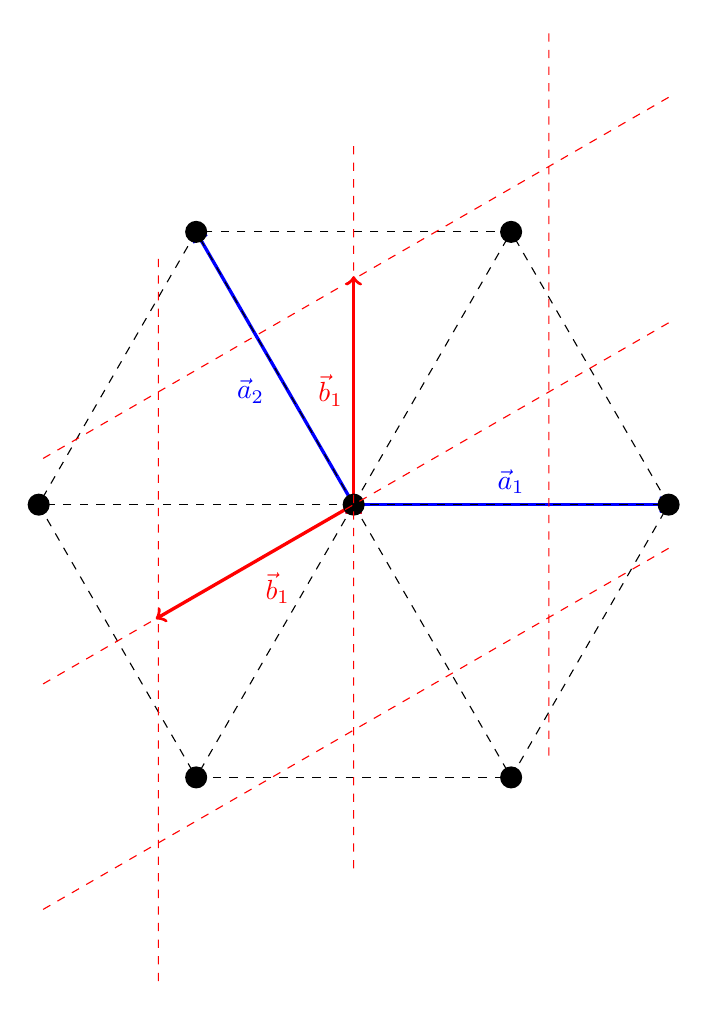
\begin{tikzpicture}[scale=2]
\foreach \i in {1,2}{
  \draw[->, blue, very thick] (0,0) edge["$\vec{a}_\i$"] (120*\i-120:2cm);}
\draw[->, red, very thick] (0,0) edge["$\vec{b}_1$"] (0,{0.8*pi/sqrt(3)});
\draw[->, red, very thick] (0,0) edge["$\vec{b}_1$"] (-0.4*pi,{-0.4*pi/sqrt(3)});
%\foreach \x in {-2,...,2}{
  %\foreach \y in {-1,0,1}{
    %\draw[red, dashed] (0,0) to (\x,\y);}}
\foreach \i in {0,...,5}{
  \draw[dashed] (60*\i:2cm) -- ({60*(\i+1)}:2cm);
  \draw[dashed] (0,0) -- (60*\i:2);
  \fill (60*\i:2) circle (0.07);}
\fill (0,0) circle (0.07);
\pgftransformcm{0}{2/sqrt(3)}{-1}{-1/sqrt(3)}{\pgfpoint{0}{0}}
  \draw[dashed, red] (-2,-2) grid[step=1.24] (2,2);
\end{tikzpicture}
\caption{Hexagonales Gitter mit Gittervektoren}
\label{figure:Hexagonales Gitter mit Gittervektoren}
\end{figure}\newpage
Die in (\ref{figure:hexagonal:WignerSeitz und Brillouin}) rot schattierte Fläche entspricht zwölf Mal der blau umrandeten Fläche. Also ist $A_\tecxt\text{rot}=12\cdot \frac{1}{2}\cdot\frac{1}{2}\cdot\frac{\sqrt{3}}{6}=\frac{\sqrt{3}}{2}$.
\begin{figure}[h!]
\centering
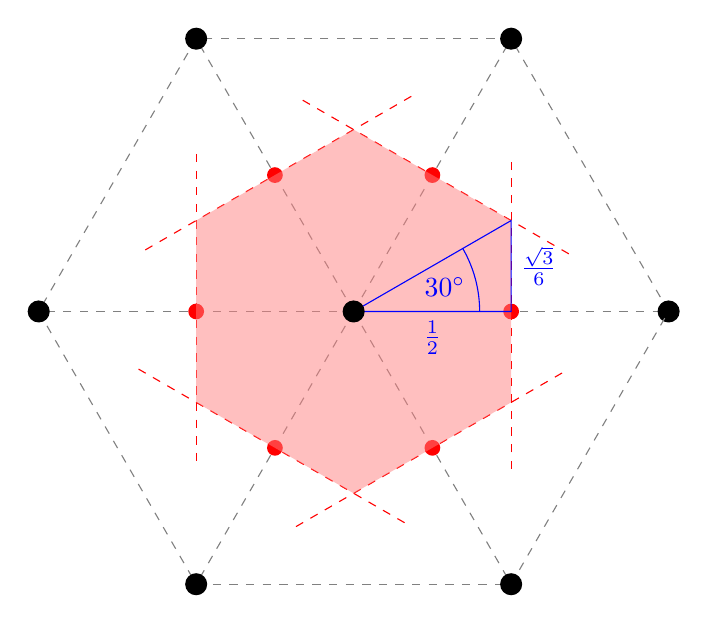
\begin{tikzpicture}[scale=2]
\foreach \i in {0,...,5}{
  \coordinate (\i) at (60*\i:2);
  \draw[dashed, gray] (\i) -- ({60*(\i+1)}:2);
  \coordinate (m\i) at ($(0,0)!0.5!(60*\i:2)$);
  \draw[dashed, gray] (0,0) -- (\i);
  \fill[red] (m\i) circle (0.05);
  \draw[rotate around={90:(m\i)},dashed,red] (0,0) -- (60*\i:2);
  \fill (\i) circle (0.07);}
\foreach \i in {0,...,5}
  \coordinate (w\i) at (60*\i+30:{2/sqrt(3)});
\path[fill=red!50,opacity=.5] (w0) to (w1) to (w2) to (w3) to (w4) to (w5);
\draw[blue] (0,0) -- (1,0) node[midway, below] {$\frac{1}{2}$} -- (1,{1/sqrt(3)}) node[midway, right] {$\frac{\sqrt{3}}{6}$} -- cycle;
\draw[blue] (0.8,0) arc (0:30:0.8);
\draw[blue] (15:0.6) node {30$\degree$};
\fill (0,0) circle (0.07);
\end{tikzpicture}
\caption{Wigner-Seitz Zelle und 1. Brillouin-Zone}
\label{figure:hexagonal:WignerSeitz und Brillouin}
\end{figure}\\

\section{Kubisch raumzentriertes Gitter}
Drei mögliche Vektoren sind gegeben durch 
\begin{align*}
A&=\frac{1}{2}\begin{pmatrix}
1&1&-1\\ 1&-1&-1 \\ 1&1&1
\end{pmatrix}=(\vec{a}_1,\vec{a}_2,\vec{a}_3)\numberthis\label{Primitive Gittvektoren 2}
\end{align*}
Diese entsprechen den $\vec{a}_{1,2,3}$ in (\ref{figure:Gittervektoren}).
\begin{figure}[h!]
\centering
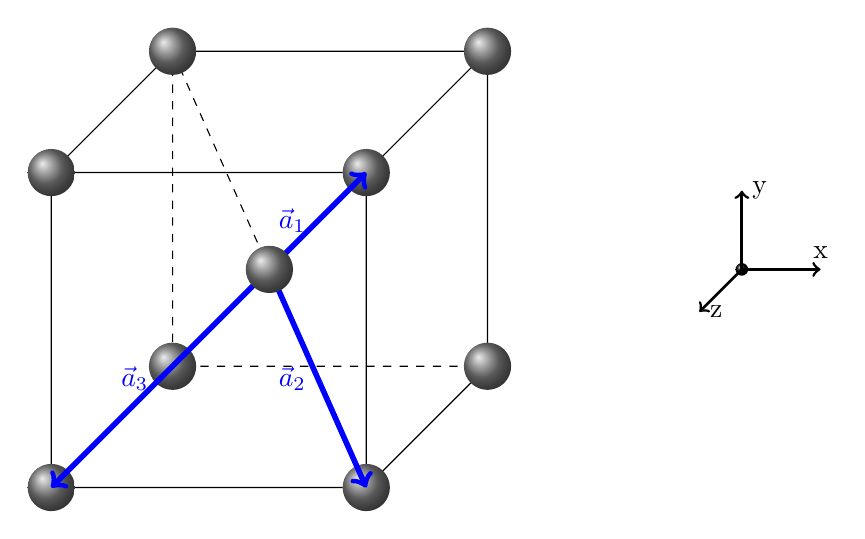
\begin{tikzpicture}[scale=2][>=stealth]
\pgfmathsetmacro{\s}{2}
\draw (0,\s,0) -- (0,0,0) -- (\s,0,0) -- (\s,\s,0) -- (0,\s,0) -- (0,\s,-\s) -- (\s,\s,-\s) -- (\s,0,-\s) -- (\s,0,0);
\draw (\s,\s,0) -- (\s,\s,-\s);
\draw[dashed] (0,0,0) -- (0,0,-\s) -- (\s,0,-\s);
\draw[dashed] (0,\s,-\s) -- (0,0,-\s) -- (1,1,-1) -- (0,\s,-\s);
\foreach \x in {0,\s}{
  \foreach \y in {0,\s}{
    \foreach \z in {0,-\s}{
      \coordinate (\x\y\z) at (\x,\y,\z);
      \shade[ball color = gray] (\x\y\z) circle (0.15);}}}
\foreach \i/\vert in {2/{\s,0,0},1/{\s,\s,0},3/{0,0,0}}
  \draw[->, blue, line width=2] (1,1,-1) -- (\vert) node[midway, left]{$\vec{a}_\i$} ;
\shade[ball color = gray] (1,1,-1) circle (0.15);
\shade[ball color = black] (4,1,-1) circle (0.04);
\foreach \i/\vect/\arg in {x/{0.5,0,0}/above,y/{0,0.5,0}/right,z/{0,0,0.7}/right}
  \draw[->, line width=1] (4,1,-1) -- ++ (\vect) node[\arg] {\i};
\end{tikzpicture}
\caption{Gittervektoren}
\label{figure:Gittervektoren}
\end{figure}\\
Die reziproken Gittervektoren berechnen sich nach $\vec{b}_1=\frac{2\pi}{\det A}\vec{a}_2\times\vec{a}_3$ (Indizes zyklisch):
\begin{align*}
B&=\frac{2\pi}{-4\cdot\frac{1}{8}}\cdot\frac{1}{4}\begin{pmatrix}
0&-2&2 \\ -2&2&0 \\ -2&0&-2
\end{pmatrix}=2\pi\begin{pmatrix}
0&1&-1 \\ 1&-1&0 \\ 1&0&1
\end{pmatrix}=(\vec{b}_1,\vec{b}_2,\vec{b}_3) \numberthis\label{Reziproke Gittervektoren 2}
\end{align*}


\end{document}